\documentclass[11pt, pdflatex]{report}
\usepackage[a4paper]{geometry}
\usepackage[french]{babel}
\usepackage[utf8]{inputenc}
\usepackage{graphicx} 
\usepackage[backend=bibtex]{biblatex}
\usepackage[T1]{fontenc}
\usepackage{listings}
\usepackage{float}
\usepackage{caption}
\usepackage{parskip}

\title{TRAVAUX PRATIQUES I.A EN SECURITE ET AIDE A LA DECISION}
\author{BOUCHHEFA Badis\and VU Nguyen Phuong Vy\and ADOUMA Hassan Brahim\and BENELAM Kamel}

\date{\today}

\begin{document}


\begin{titlepage}
    \vspace*{1em}
    \centering
    {\LARGE TRAVAUX PRATIQUES INTELLIGENCE ARTIFICIELLE ET JEUX ADVERSARIAUX EN SECURITE ET AIDE A LA DECISION\par}
    \vspace{1cm}
    {\scshape\Large JEU D'INFECTION\par}
    \vspace{1cm}
	{\Large VU Nguyen Phuong Vy - 21911658\par}
	{\Large BOUCHHEFA Badis - 21914662 \par}
	{\Large ADOUMA Hassan Brahim - 21901741\par}
	{\Large BENELAM Kamel - 21913417\par}
    \vspace{1cm}
	{\large \today \par}
    \vspace{1cm}

    \begin{figure}[H]
        \centering
        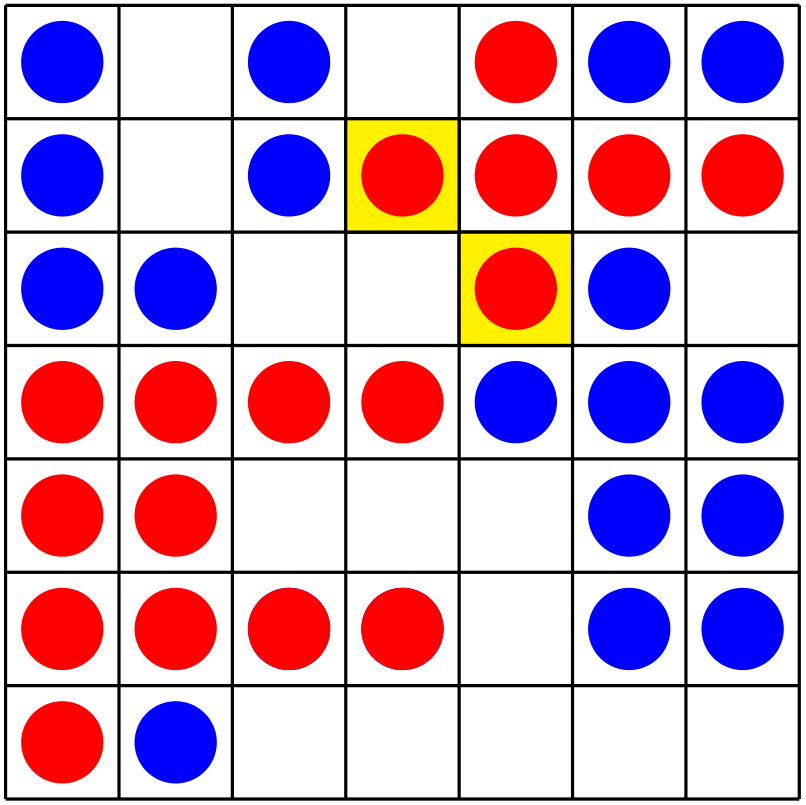
\includegraphics[width=0.5\textwidth]{capture.png}
    \end{figure}
    
\end{titlepage}

\pagebreak

\tableofcontents

\pagebreak
\section{Introduction}
Après avoir réalisé le jeu et d’implémenter tous les expérimentations nécessaires nous vous expliquons le déroulement du jeu et de ces expérimentations.

\section{Diagramme}
Voici notre diagramme de classe UML, Afin de bien simplifier et de comprendre notre code:
\begin{figure}[H]
    \centering
    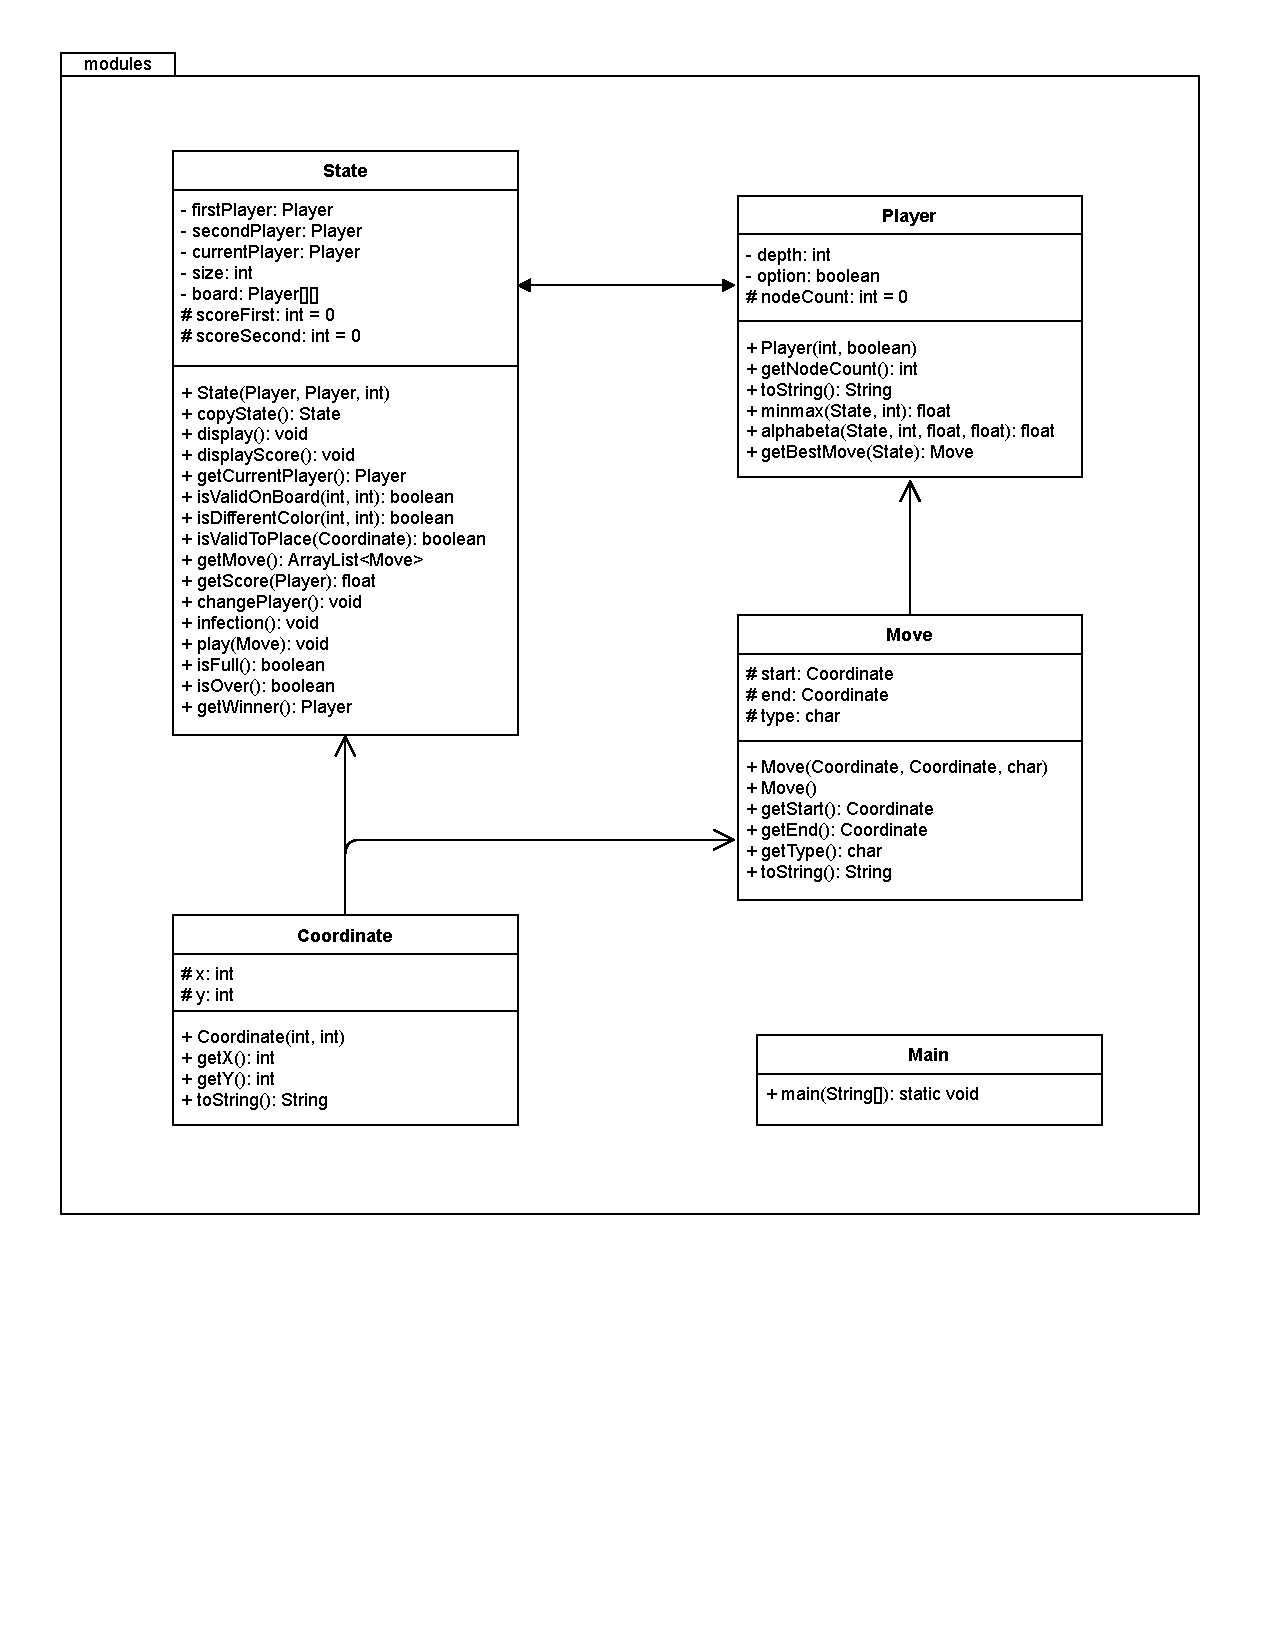
\includegraphics[width=1\textwidth]{uml.pdf}
    \vspace{-12em}
    \caption{La photo du diagramme}
\end{figure}


\section{Expérimentation}
L’expérimentation du jeux de ce jeux nécessite deux algorithmes très importants à signaler qui sont: \par

\subsection{minmax}
L’idée de cet algorithme est de développer complètement l’arbre de jeu, de noter chaque feuille possede  sa propre valeur, puis de faire remonter ces valeurs avec l’hypothèse que chaque joueur choisit le meilleur coup pour lui. \par
L’algorithme minmax amène donc à développer un nombre exponentiel des branches selon la profondeur à laquelle on s’intéresse. \par
Le graphe ci-dessous représente le nombre de nœuds explorés par minmax :

\begin{figure}[H]
    \centering
    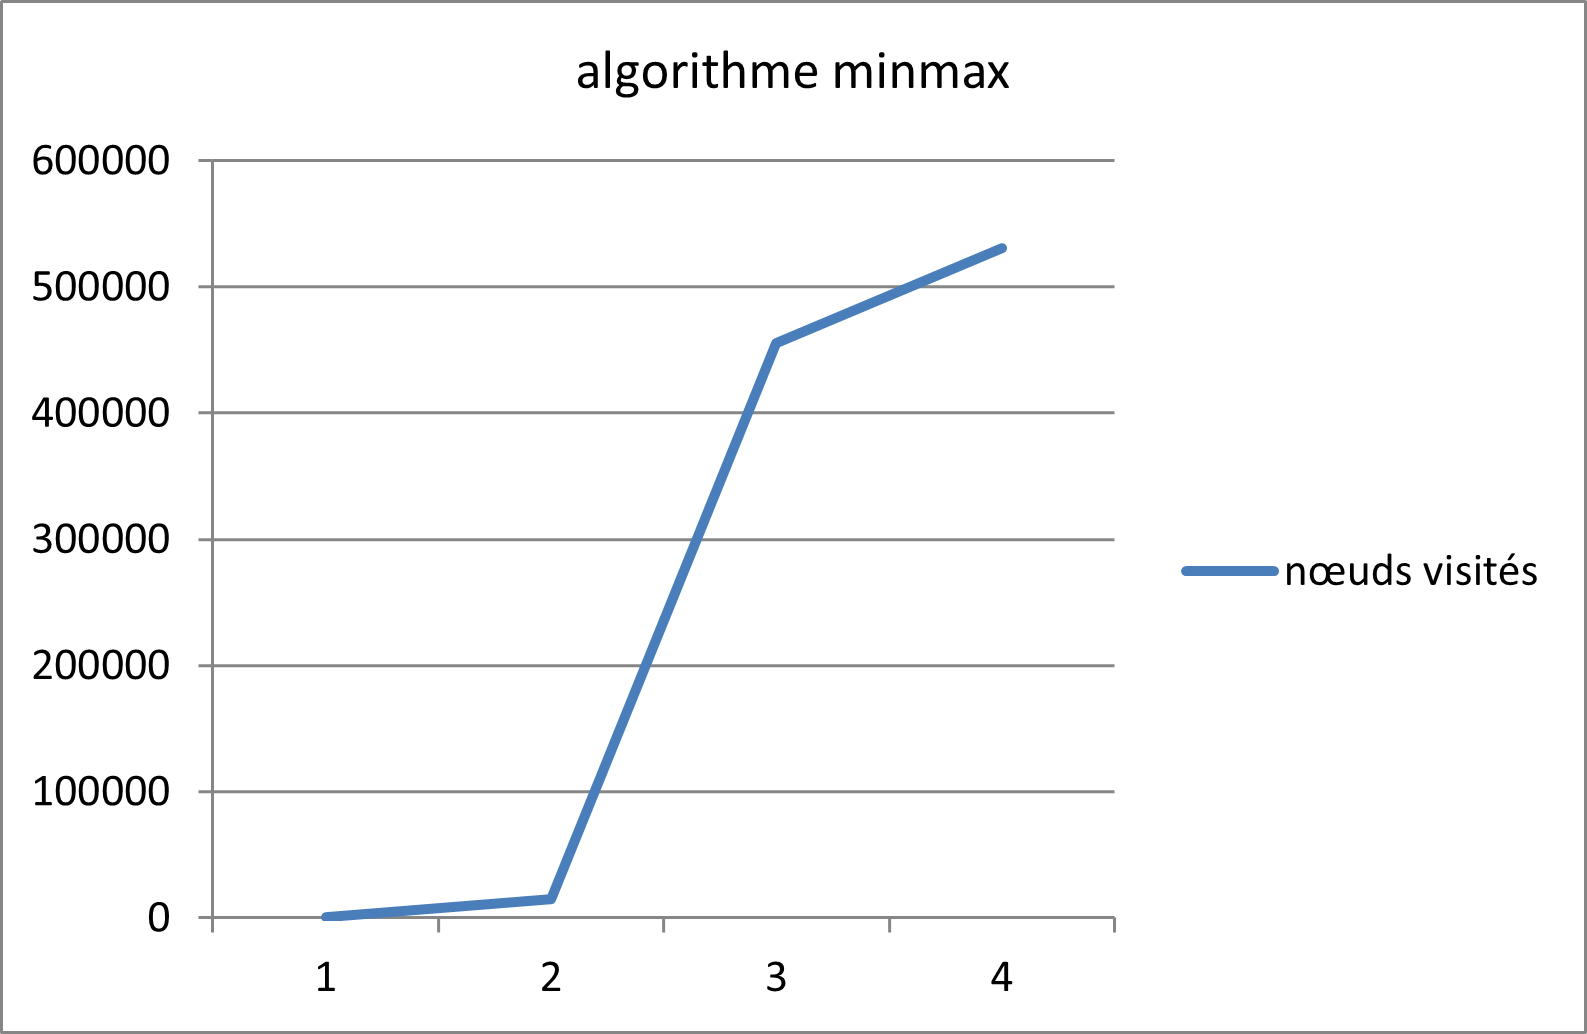
\includegraphics[width=0.6\textwidth]{minmax1.png}
    \caption{Courbe de l'algorithme minmax avec profondeur à 4}
\end{figure}

\begin{figure}[H]
    \centering
    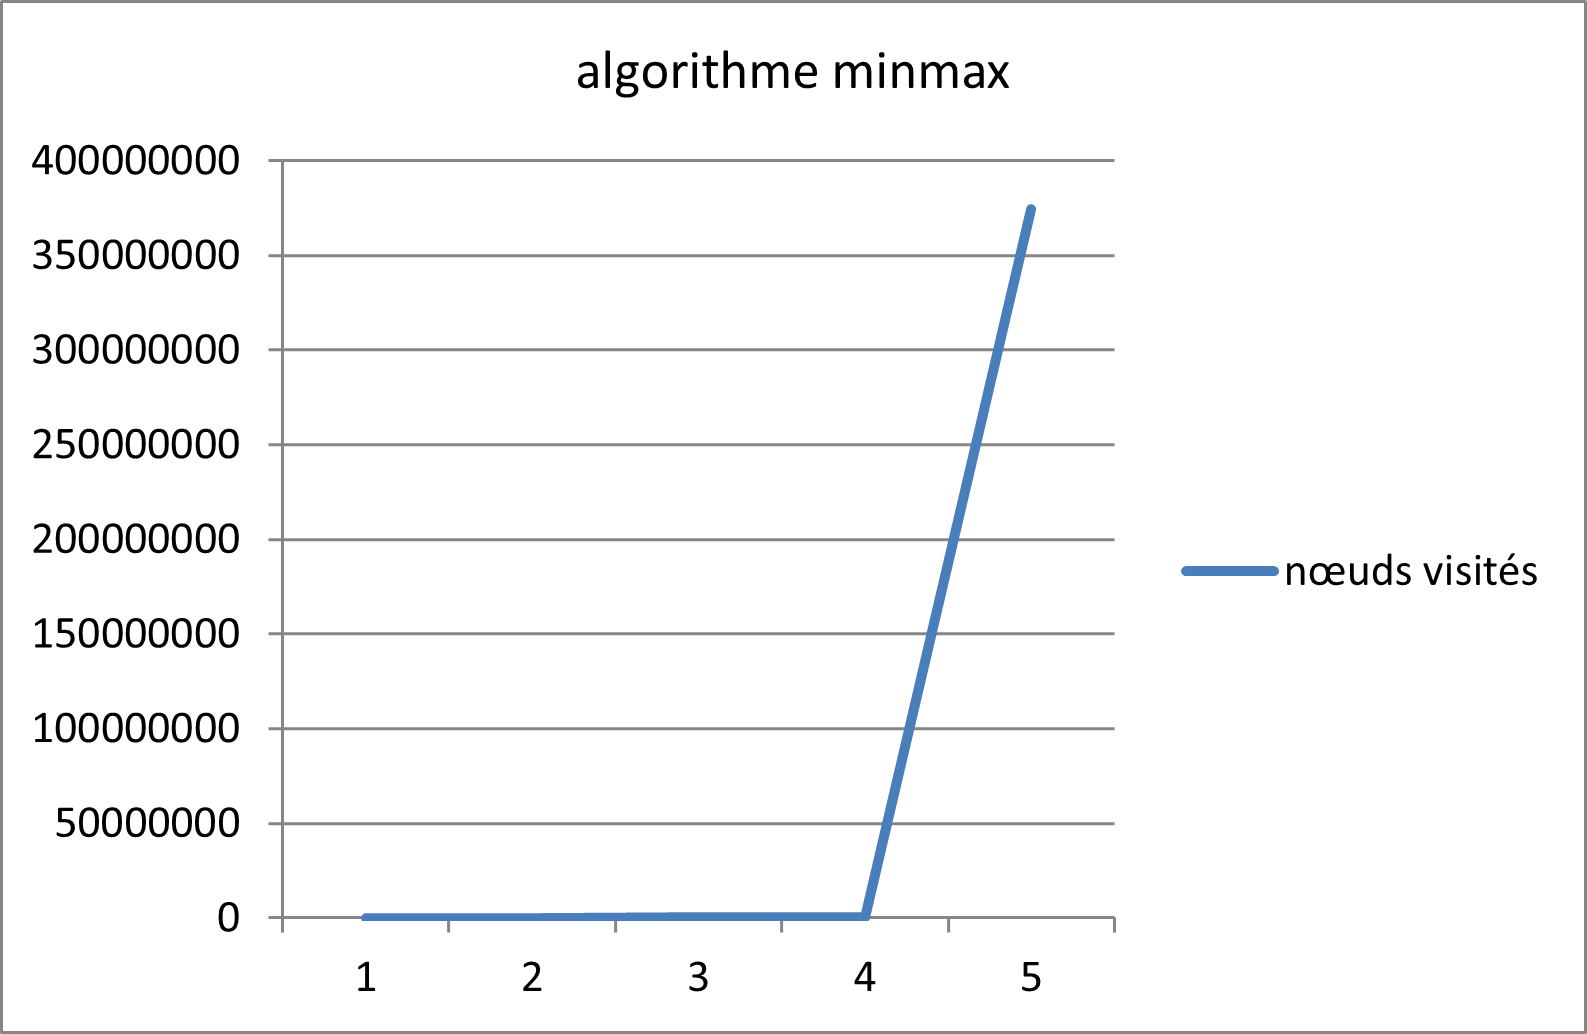
\includegraphics[width=0.6\textwidth]{minmax2.png}
    \caption{Courbe de l'algorithme minmax avec profondeur à 5}
\end{figure}

\newpage
\subsection{alphabeta}
Cet algorithme n’est autre qu’une amélioration du minmax sur sa version negamax et l’idée de cet algorithme est d’élaguer certaines branches de l’arbre, car elle coupe les branches inutiles de l’arbre qui sont pour le pion concerné des branches perdantes.\par
Le graphe suivant représentant le nombre de nœuds explorés par alphabeta :\par

\begin{figure}[H]
    \centering
    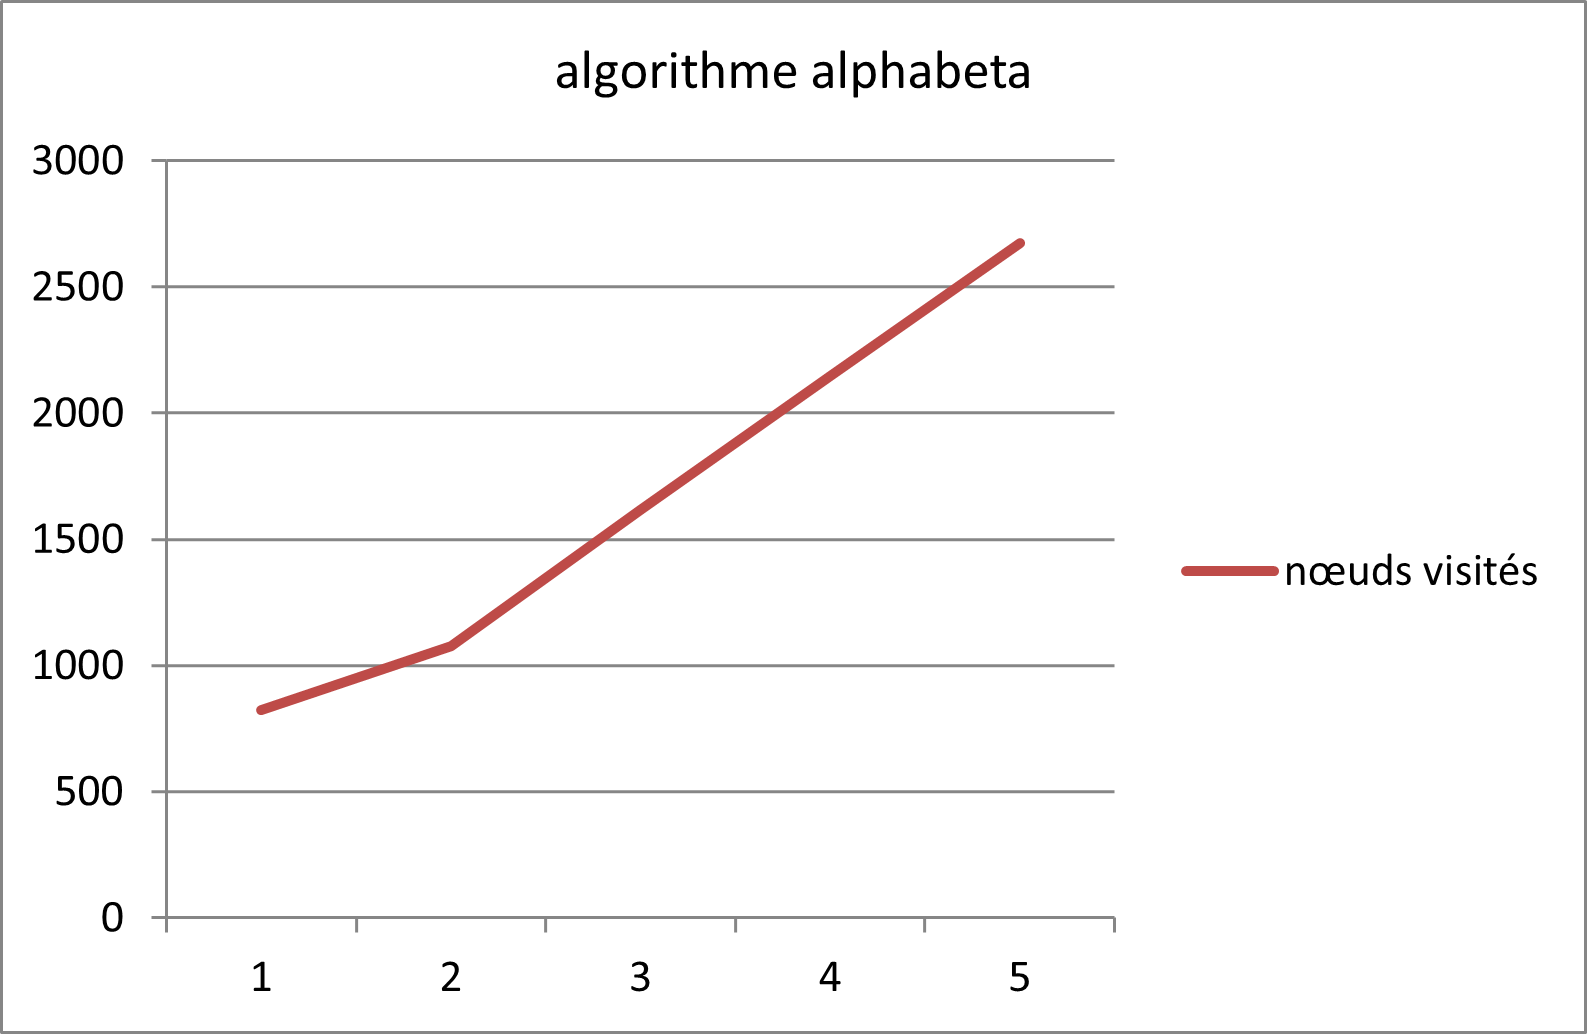
\includegraphics[width=0.8\textwidth]{alphabeta.png}
    \caption{Courbe de l'algorithme alphabeta}
\end{figure}

Voici le tableau qui résume les deux courbes :
 
 \begin{center}
    \begin{tabular}{|l|l|l|}\hline   
    Profondeur&      minmax&      alphabeta      \\\hline
    1&      822&      822      \\\hline
    2&      14788&      1078      \\\hline
    3&      455305&      1615      \\\hline
    4&      530578&      2147      \\\hline
    5&      374174846 (très grand nombre)&      2675      \\\hline
    \end{tabular}
\end{center}

\newpage
\section{Raisonement de la profondeur}
Afin d’identifier l’intérêt du raisonnement en profondeur et de mieux analyser les algorithmes minmax et alphabeta. On fixe la taille de la grille (7 x 7)  et une profondeur de raisonnement pour les deux joueurs. Car on fixe la profondeur du premier joueur à 2 et on change pour le deuxième joueur, on a utilisé l’algorithme alphabeta qui car il est le plus simple. Les résultats sont :  \par

\begin{center}
    \begin{tabular}{|l|l|l|}\hline   
        Profondeur de Joueur 1\up{er}&      Profondeur de Joueur 2\up{ème}&      Gagnant      \\\hline
    2&      1&      Joueur 1\up{er}      \\\hline
    2&      2&      Joueur 1\up{er}      \\\hline
    2&      3&      Joueur 1\up{er}      \\\hline
    2&      4&      Joueur 1\up{er}      \\\hline
    2&      5&      Joueur 1\up{er}      \\\hline
    \end{tabular}
\end{center}

On remarque que le premier joueur a gagné toutes les parties dans ce cas mais dans le cas où la profondeur du premier joueur change donc la gagnant change aussi.\par

\section{Conclusion}
En conclusion, ce jeu marchera d’après la profondeur donner et nous pouvont voir à travers des deux courbes que l’algorithme alphabeta et plus simple que minmax car il est optimal en calcul des nœuds visités. 

\end{document}